\documentclass[12pt]{article}
\usepackage{amsmath, amssymb, amsthm}
\usepackage{mathtools}
\usepackage{graphicx}
\usepackage{float}
\usepackage{hyperref}
\usepackage{xcolor}
\usepackage{listings}
\usepackage{geometry}
\usepackage{algorithm}
\usepackage{algpseudocode}
\usepackage{tikz}
\usepackage{longtable}
\usepackage{circuitikz}
\usepackage{comment}
\usepackage[section]{placeins}

% Page Setup
\geometry{a4paper, margin=1in}
\setlength{\intextsep}{10pt} % Space between text and floats
\bibliographystyle{IEEEtran}

% Custom Commands
\newcommand{\vecb}[1]{\mathbf{#1}}
\newcommand{\brak}[1]{\ensuremath{\left(#1\right)}}
\newcommand{\cbrak}[1]{\ensuremath{\left\{#1\right\}}}
\newcommand{\abs}[1]{\left\vert#1\right\vert}
\newcommand{\norm}[1]{\left\lVert#1\right\rVert}

\begin{document}
\title{}
\author{}
%{\let\newpage\relax\maketitle}

\section{Convergence of fourier series for the square wave with duty ratio $\alpha$}

\subsection{Dirichlet Conditions for Fourier Series Convergence}

For a Fourier series to be pointwise convergent, the function must satisfy the followin Dirichlet conditions,

\begin{enumerate}
\item The periodic signal must have a finite number of maxima and minima over one period
\item The periodic signal must have a finite number of discontinuities over one period
\item The periodic signal must be absolutely integrable over one period
\end{enumerate}

Let's define our square wave function with period $T$ and duty ratio $\alpha$ $(0 < \alpha < 1)$ as,

\begin{equation}
f(t) =
\begin{cases}
A, & 0 \leq t < \alpha T \\
0, & \alpha T \leq t < T
\end{cases}
\end{equation}

with $f(t+T) = f(t) \; \forall \; t$.

\subsubsection{Checking Dirichlet Conditions}

\begin{enumerate}
\item \textbf{Finite maxima and minima}: The square wave has exactly one maximum and one minimum in one period. At $t = 0$, the function jumps to its maximum value $A$ and at $t = \alpha T$, it drops to its minimum value $0$.

\item \textbf{Finite discontinuities}: The square wave has exactly two discontinuities per period. These occur at $t = 0$ and $t = \alpha T$ where the function value changes abruptly.

\item \textbf{Absolute integrability}: The integral of $|f(t)|$ over one period is:
\begin{align}
\int_0^T |f(t)| dt &= \int_0^{\alpha T} |A| dt + \int_{\alpha T}^T |0| dt \\
&= A \cdot \alpha T
\end{align}
This is finite, so the third condition is satisfied.
\end{enumerate}

Since all three Dirichlet conditions are met, the Fourier series of the square wave with duty ratio $\alpha$ is pointwise convergent.

\subsection{Convergence Behavior}

According to the Fourier Convergence Theorem, the Fourier series converges to:
\begin{itemize}
\item The function value $f(t)$ at all points where $f(t)$ is continuous
\item The average of the left and right limits $\frac{1}{2}[f(t^+) + f(t^-)]$ at points of discontinuity
\end{itemize}

For our square wave, at the discontinuities ($t = 0$ and $t = \alpha T$), the Fourier series converges to,
\begin{equation}
\frac{1}{2}(A + 0) = \frac{A}{2}
\end{equation}

\subsection{Gibbs phenomenon and fourier series representation}

The Fourier series for this square wave is,

\begin{align}
f(t) &= A\alpha + \sum_{n=1}^{\infty} \frac{A}{n\pi} \sin(n\pi\alpha) \cos\left(\frac{2\pi nt}{T}\right) + \sum_{n=1}^{\infty} \frac{A}{n\pi} [1-\cos(n\pi\alpha)] \sin\left(\frac{2\pi nt}{T}\right)
\end{align}

As we include more terms ($N \rightarrow \infty$), the partial sums of this series converge to the square wave at all points except at the discontinuities, where they converge to the average of the left and right limits.

This pointwise convergence is visually evident when plotting successive partial sums, showing how the approximation improves as more terms are added.
\newline

An interesting observation is that around the discontinuities, oscillations (overshoots and undershoots) are seen even at higher $N$ values. As $N$ increases, the oscillations gradually become narrower, although they do not disappear.
This is known as the \textbf{Gibbs Phenomenon}

\begin{figure*}[!htb]
    {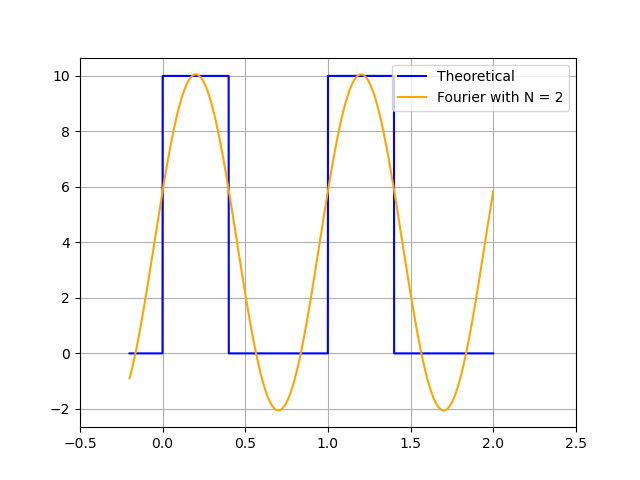
\includegraphics[ width=0.5\textwidth]{./figs/convergence_n2.png}}
    \hspace{\fill}
    {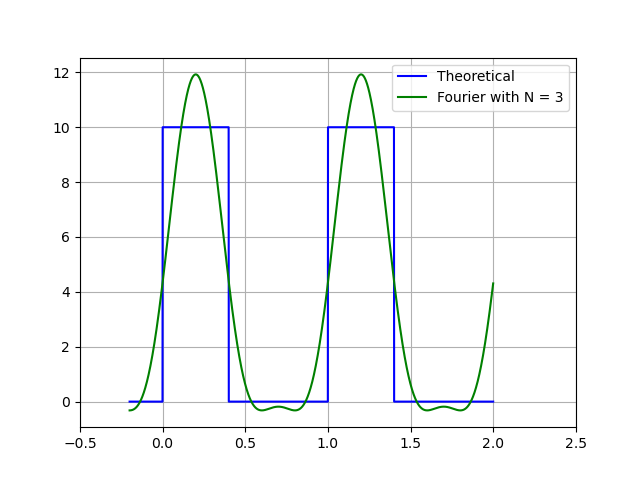
\includegraphics[ width=0.5\textwidth]{./figs/convergence_n3.png}}
\end{figure*}

\begin{figure*}[!htb]
    {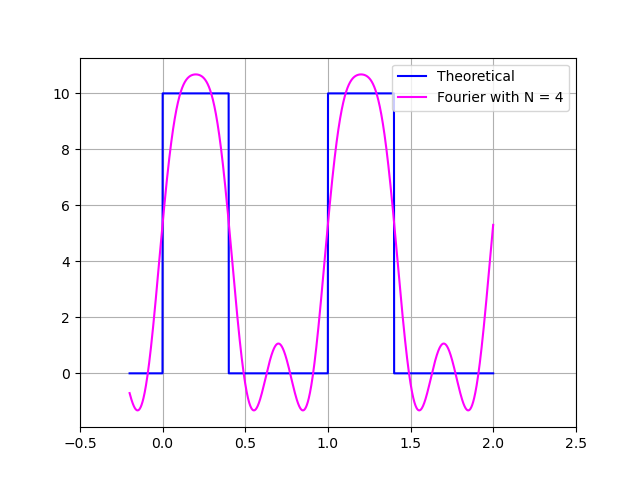
\includegraphics[ width=0.5\textwidth]{./figs/convergence_n4.png}}
    \hspace{\fill}
    {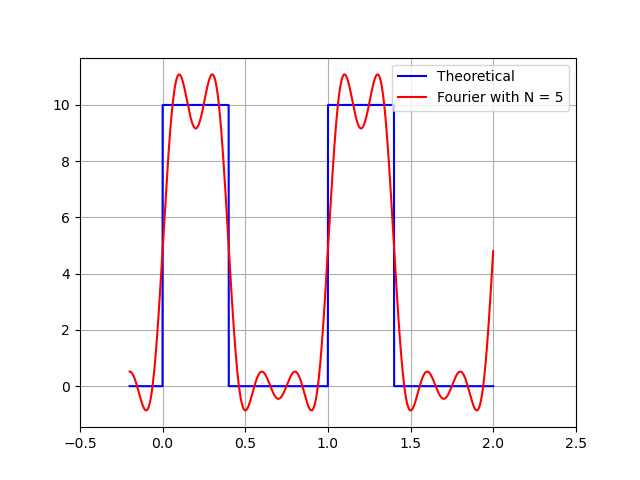
\includegraphics[ width=0.5\textwidth]{./figs/convergence_n5.png}}
\end{figure*}

\begin{figure*}[!htb]
    {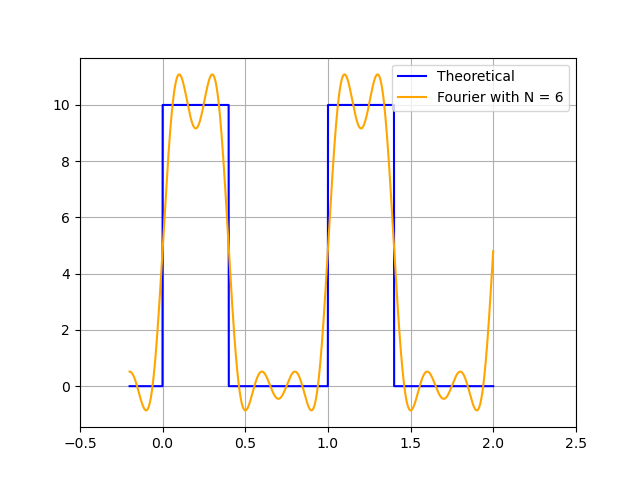
\includegraphics[ width=0.5\textwidth]{./figs/convergence_n6.png}}
    \hspace{\fill}
    {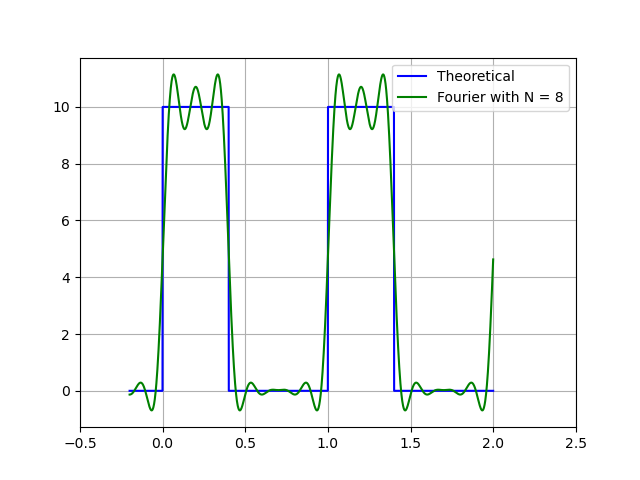
\includegraphics[ width=0.5\textwidth]{./figs/convergence_n8.png}}
\end{figure*}

\begin{figure*}[!htb]
    {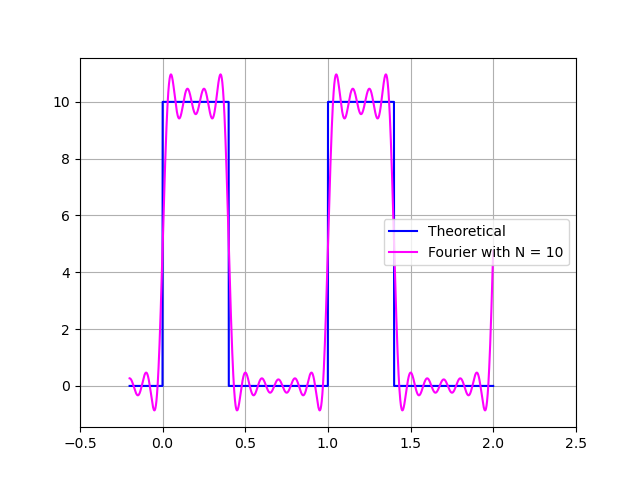
\includegraphics[ width=0.5\textwidth]{./figs/convergence_n10.png}}
    \hspace{\fill}
    {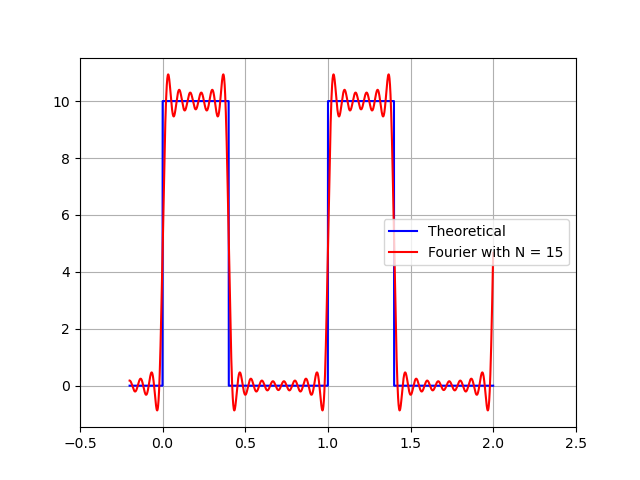
\includegraphics[ width=0.5\textwidth]{./figs/convergence_n15.png}}
\end{figure*}

\begin{figure*}[!htb]
    {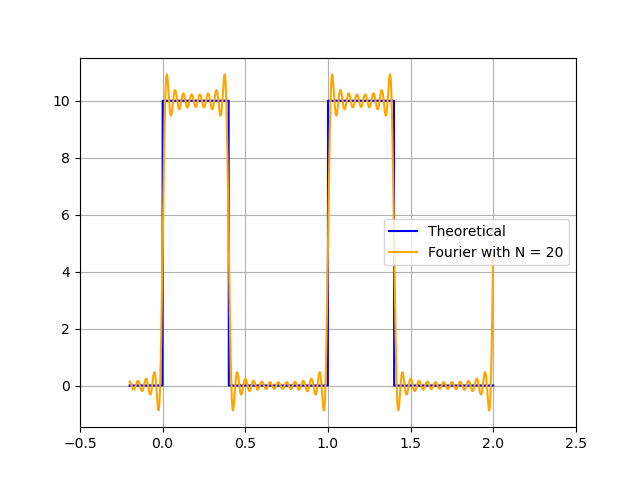
\includegraphics[ width=0.5\textwidth]{./figs/convergence_n20.png}}
    \hspace{\fill}
    {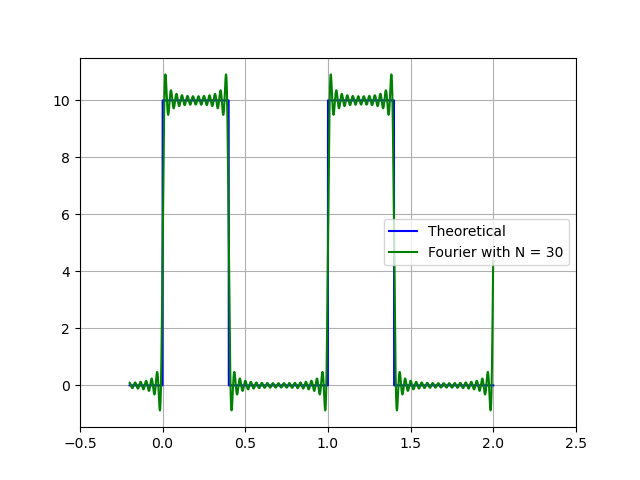
\includegraphics[ width=0.5\textwidth]{./figs/convergence_n30.png}}
\end{figure*}

\begin{figure*}[!htb]
    {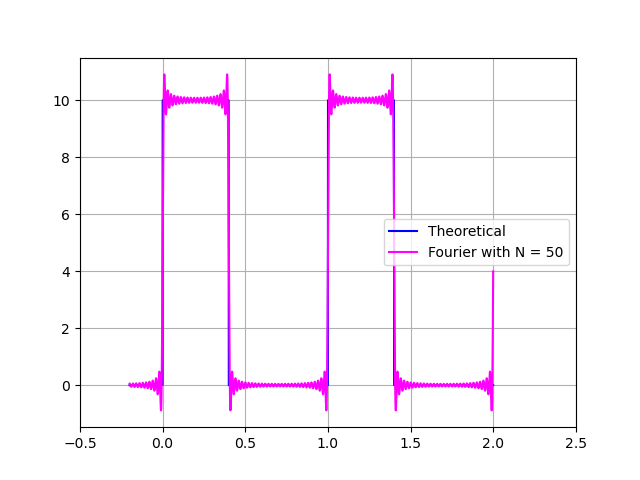
\includegraphics[ width=0.5\textwidth]{./figs/convergence_n50.png}}
    \hspace{\fill}
    {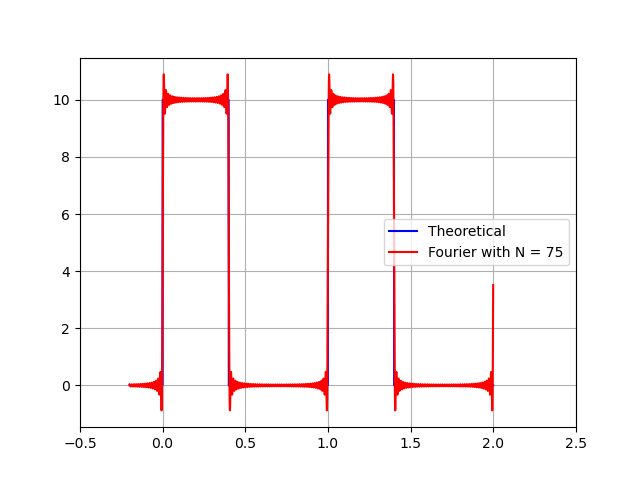
\includegraphics[ width=0.5\textwidth]{./figs/convergence_n75.png}}
\end{figure*}

\begin{figure*}[!htb]
    {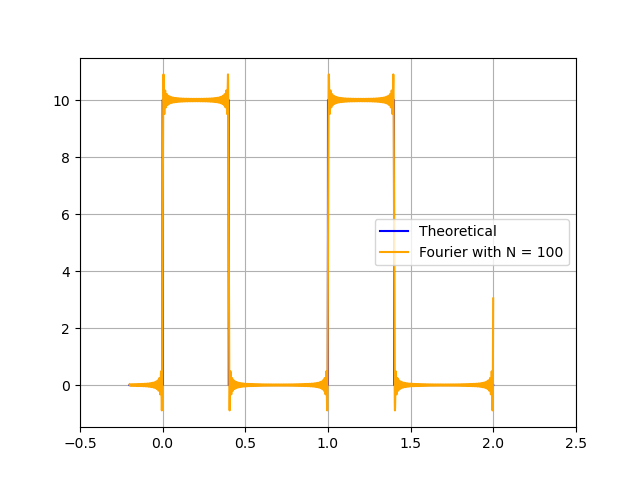
\includegraphics[ width=0.5\textwidth]{./figs/convergence_n100.png}}
    \hspace{\fill}
    {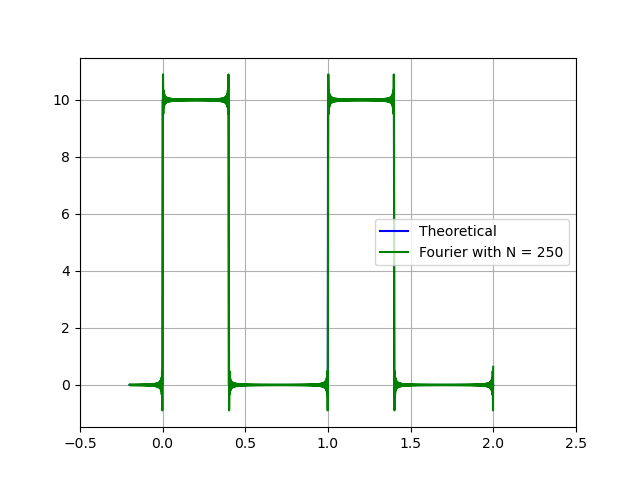
\includegraphics[ width=0.5\textwidth]{./figs/convergence_n250.png}}
\end{figure*}

\begin{figure*}[!htb]
    {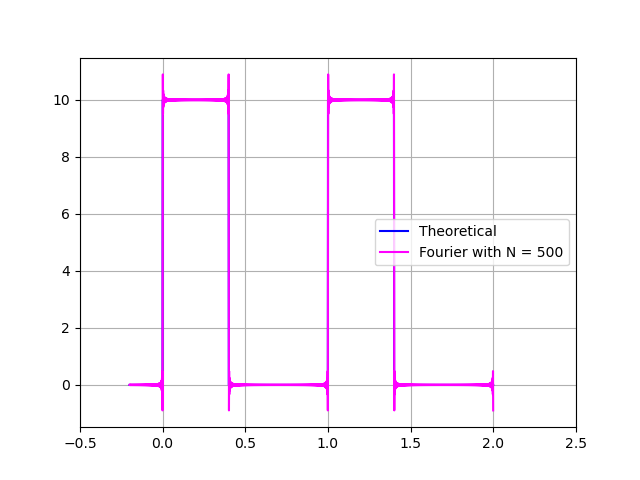
\includegraphics[ width=0.5\textwidth]{./figs/convergence_n500.png}}
    \hspace{\fill}
    {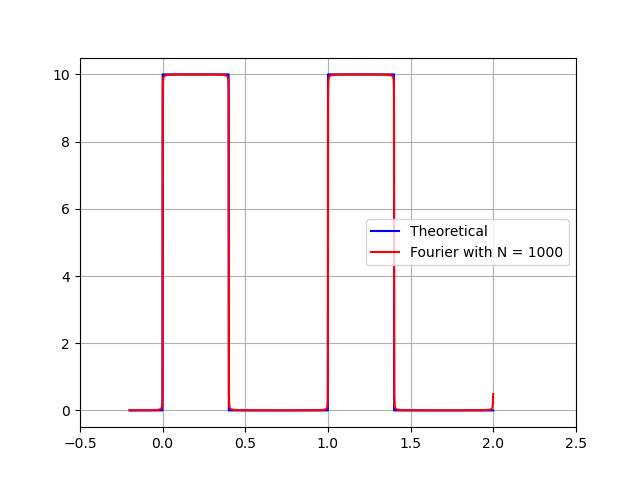
\includegraphics[ width=0.5\textwidth]{./figs/convergence_n1000.png}}
\end{figure*}

\end{document}
